% Exemplo de relatório técnico do IC
% Criado por P.J.de Rezende antes do Alvorecer da História.
% Modificado em 97-06-15 e 01-02-26 por J.Stolfi.
% Last edited on 2003-06-07 21:12:18 by stolfi

% modificado em 1o. de outubro de 2008

\documentclass[11pt,twoside]{article}
\usepackage{techrep-ic}

%%% SE USAR INGLÊS, TROQUE AS ATIVAÇÕES DOS DOIS COMANDOS A SEGUIR:
\usepackage[brazil]{babel}
%% \usepackage[english]{babel}

%%% SE USAR CODIFICAÇÃO LATIN1, TROQUE AS ATIVAÇÕES DOS DOIS COMANDOS A
%%% SEGUIR:
%% \usepackage[latin1]{inputenc}
\usepackage[utf8]{inputenc}
\usepackage[dvips]{graphicx}

\begin{document}

%%% PÁGINA DE CAPA %%%%%%%%%%%%%%%%%%%%%%%%%%%%%%%%%%%%%%%%%%%%%%%
% 
% Número do relatório
\TRNumber{007}

% DATA DE PUBLICAÇÃO (PARA A CAPA)
%
\TRYear{12}  % Dois dígitos apenas
\TRMonth{09} % Numérico, 01-12

% LISTA DE AUTORES PARA CAPA (sem afiliações).
\TRAuthor{R. Barboza Jr \and D. C. S. Lucas \and A. S. Ferreira}

% TÍTULO PARA A CAPA (use \\ para forçar quebras de linha).
\TRTitle{Box \\An IA-32 Process Emulator}

\TRMakeCover

%%%%%%%%%%%%%%%%%%%%%%%%%%%%%%%%%%%%%%%%%%%%%%%%%%%%%%%%%%%%%%%%%%%%%%
% O que segue é apenas uma sugestão - sinta-se à vontade para
% usar seu formato predileto, desde que as margens tenham pelo
% menos 25mm nos quatro lados, e o tamanho do fonte seja pelo menos
% 11pt. Certifique-se também de que o título e lista de autores
% estão reproduzidos na íntegra na página 1, a primeira depois da
% página de capa.
%%%%%%%%%%%%%%%%%%%%%%%%%%%%%%%%%%%%%%%%%%%%%%%%%%%%%%%%%%%%%%%%%%%%%%

%%%%%%%%%%%%%%%%%%%%%%%%%%%%%%%%%%%%%%%%%%%%%%%%%%%%%%%%%%%%%%%%%%%%%%
% Nomes de autores ABREVIADOS e titulo ABREVIADO,
% para cabeçalhos em cada página.
%
\markboth{Barboza, Lucas e Ferreira}{Box}
\pagestyle{myheadings}

%%%%%%%%%%%%%%%%%%%%%%%%%%%%%%%%%%%%%%%%%%%%%%%%%%%%%%%%%%%%%%%%%%%%%%
% TÍTULO e NOMES DOS AUTORES, completos, para a página 1.
% Use "\\" para quebrar linhas, "\and" para separar autores.
%
\title{Box: An IA-32 Process Emulator}

\author{
 Roberto Barboza Jr
   \thanks{RA: 035712, rbarboza@gmail.com} \and
 Divino C. S. Lucas
   \thanks{RA: 115121, divcesar@gmail.com} \and
 Anderson Soares Ferreira
   \thanks{RA: 974530, asferreira.ferreira@gmail.com}
}

\date{}

\maketitle

%%%%%%%%%%%%%%%%%%%%%%%%%%%%%%%%%%%%%%%%%%%%%%%%%%%%%%%%%%%%%%%%%%%%%%%%%%%%%%%%%

\begin{abstract} 
 As máquinas virtuais são ferramentas amplamente utilizadas para resuloção de diversas problemas computacionais e podem ser classificadas de diversas formas, de acordo com sua implementação.
 Como forma de ampliar a compreensão das implicações resultantes das diferentes características de implementação dos diversos tipos de máquinas virtuais, este trabalho apresenta uma comparação de desempenho entre máquinas virtuais interpretadas de sistema e de processo.
 Para tanto, o presente estudo faz a comparação das ferramentas \emph{Bochs}, um gerenciador de máquinas virtuais de sistema, e um gerenciador para máquinas virtuais de processo chamodo \emph{Box}, desenvolvido a partir da ferramenta anterior especificamente para esse estudo.
\end{abstract}

\section{Introdução}
% aqui vamos dar introdução ao assunto de máquinas virtuais
% falar sobre os modos de emulação 
% falar que máquinas virtuais podem ser usadas para pesquisa
% pois permitem fazer analise do código, etc.
% comentar brevemente qual ẽ o nosso objetivo no projeto.

Uma Máquina Virtual (MV) é uma plataforma versátil que pode ser empregada para resolver diversos problemas na área de computação. 
Uma MV pode ser vista como uma camada de software utilizada para prover a integração entre duas interfaces distintas.
As interfaces descritas podem ser tanto \emph{Application Binary Interface} (ABI) em máquinas virtuais de processo, quanto \emph{Instruction Set Architecture} (ISA) em MV de sistema.
Nesse sentido, tais tecnologias ocupam uma posição estratégica que pode ser explorada de diversas formas:
Na emulação de arquiteturas diferentes, permitindo que aplicações escritas para um plataforma específica possa ser executada em outra; para simulação e instrumentação de sistemas ou aplicações; ou otimização dinâmica de binários.

Duas abordagens são frequentemente empregadas para implementar a emulação em uma máquina virtual: interpretação e tradução.
Uma MV que emprega interpretação utiliza funções para simular o comportamento de cada instrução da aplicação sendo emulada. 
O processo de tradução porém, emprega técnicas da área de compiladores para produzir um código binário nativo (possívelmente otimizado) equivalente aquele da aplicação sendo emulada.
É comum encontrarmos MV que, visando maximizar o desempenho, empregam estas abordagens em conjunto.

Nesse texto descrevemos uma proposta de implementação de uma máquina virtual de processo que emprega interpretação como forma de emulação. 
O objetivo desta MA não é otimizar a execução da aplicação sendo emulada mas sim, criar uma infraestrutura que permita a realização de experimentos voltados para a área de máquinas virtuais.
   
\section{Objetivos}
% Aqui vamos apresentar nosso objetivo principal que é desenvolver
% uma máquina virtual de processo que emprega interpretação para
% fazer a emulação do sistema.
% 
% precisamos também adicionar como objetivo a análise do desempenho
% da nossa implementação em relação ao Bochs.

As diferentes implementações de MV apresentam características que determinam seu desempenho e aplicabilidade.
Por exemplo, implementações interpretadas tem como principal característica a portabilidade de código, permitindo que sejam utilizadas em diferentes plataformas. 
Em contrapartidada, apresentam desempenho inferior à implementações que utilizam tradução dinâmica de binários.

Neste contexto, são escassos os dados sobre os custos (recursos computacionais e desempenho) para executar uma máquina virtual de sistema e de processos. 
Visto que a primeira apresenta o overhead de emular todos os subsistemas de um computador real e ainda executar um sistema operacional completo, enquanto que na máquina virtual de processos apenas emula o sistema operacional.
Desta forma, o objetivo geral deste trabalhor é apresentar uma comparação sobre o desempenho destes dois tipos de máquinas virtuais.
Como forma de atingir o objetivo descrito, os seguintes objetivos específicos serão desenvolvidos:

\begin{itemize}
 \item Implementação de uma máquina virtual interpretada de processos a partir do emulador de sistemas Bochs;
 \item Implementação de mecanismos de otimização da execução como forma de melhorar o desempenho do ambiente virtualizado.
 \item Aplicação sistemáticas de teste e medição e análise de desempenho do ambiente virtualizado de sistema (\emph{Bochs}) e no ambiente proposto (\emph{Box});
\end{itemize} 

Na próxima seção apresentamos os trabalhos relacionados a este projeto.
\section{Fundamentação Teórica}
 % acho que esse nome não está bom...
 \subsection{Técnicas de Interpretação}

 % acham que precisamos incluir esta subsecao?
 % penso em colocar aqui um comentário sobre o ELF e sobre as syscalls do linux
 \subsection{Application Binary Interface}

\section{Levantamento Bibliográfico}
% Aqui devemos comentar sobre os trabalhos relacionados ao nosso
% podemos comentar sobre o Bochs, o PIN e o HDTrans por exemplo.
% comentar no que nosso sistema é diferente do deles.

\subsection{Máquinas Virtuais}
O Bochs \cite{bochs} é uma máquina virtual de sistema com suporte a emulação de diversos processadores da família x86 32 e 64 bits. 
Ele preza por portabilidade, e nesse sentido utiliza interpretação como técnica de emulação. Para reduzir o overhead de interpretação, o Bochs utiliza as técnicas de pre-decoding \cite{smith} e threaded-interpretation \cite{smith}.
O sistema que estamos propondo se diferencia do Bochs por ser voltado à emulação de processos e não de sistemas.

O Pin \cite{pin} é uma máquina virtual de processo que emula os ISAs IA-32 e x86-64. 
Ele é uma ferramenta de código fechado e possui versões tanto para Windows como para Linux, sendo reconhecido por prover uma rica API para criação de ferramentas (Pintools) para análise do comportamento dinâmico de aplicações. 
O Box diferencia-se do PIN por ser uma máquina virtual de código aberto e utilizar interpretação como técnica de emulação.
Em contrapartida, os sistemas se assemelham no aspecto de proverem uma interface para instrumentação de binários e serem emuladores \emph{same-ISA}~\footnote{As duas interfaces da máquina virtual são iguais.}.

O HDTrans \cite{hdtrans} é uma máquina virtual de processo para a arquitetura IA-32.
O HDTrans difere do Bochs e do PIN por empregar tradução de binários como técnica de emulação.
No entanto, o HDTrans abre mão de empregar otimizações no código traduzido (o que geralmente é feito para amortizar o overhead de tradução) em favor da implementação de uma tradução simples e rápida.
O Box diferencia-se do HDTrans por empregar interpretação de binários.

O Dynamo \cite{dynamo} é uma máquina virtual de processo para a arquitetura do HP PA-800. 
Diferentemente do PIN, Bochs e HDTrans, o Dynamo é uma máquina virtual cujo objetivo é otimizar a execução do programa sendo emulado.
Para tanto o Dynamo emprega uma combinação das técnicas de interpretação e emulação. 
O sistema inicialmente interpreta o código da aplicação sendo emulada. 
Uma vez que uma região é declarada como quente, o Dynamo aplica otimizações nesta região e salva o código otimizado em uma cache de traduções. 
Subsequentes invocações do trecho de código original serão emuladas utilizando o código traduzido. 
O Box diferencia-se do Dynamo por não ter o foco na otimização de binários mas sim em ser um sistema que prove uma interface simples para 
instrumentação de binários.

O IA-32 EL \cite{ia32el} é uma máquina virtual de processos com o objetivo de suportar a execução de aplicações IA-32 em processadores da família IA-64.
De forma similar ao Dynamo, o IA-32 EL emprega uma abordagem de emulação em duas etapas, porém as duas etapas realizam tradução de código. 
Inicialmente o IA-32 EL efetua a tradução de código em uma granularidade de bloco básico.
Durante essa tradução, código de instrumentação é inserido para detectar blocos básicos que são frequentemente executados. 
Quando um número mínimo de blocos básicos é identificado, o sistema forma uma região de código envolvendo esses blocos básicos, os otimiza e posteriormente salva em uma cache de traduções. 
Execuções subsequentes desses blocos básicos usam a tradução otimizada. 
O Box diferencia-se do IA-32 EL por não fazer tradução de binários.

StarDBT \cite{stardbt} é uma máquina virtual de pesquisa capaz de fazer traduções de aplicações compiladas para x86 32/64 bits para execução em hardware x86 32 bits.
De forma similar ao IA-32 EL, o StarDBT é um tradutor em duas fases. 
Regiões de código que são infrequentemente executadas são traduzidas utilizando um tradutor simples e rápido, enquanto regiões de código que são frequentemente executadas são traduzidas empregando otimizações de código e posteriormente persistidas em uma cache de traduções. 
O Box diferencia-se do StarDBT por ser capaz de traduzir apenas binários de 32 bits, compilados para Linux e não empregar tradução de binários.

\section{Infraestrutura de Pesquisa}
% Aqui explicamos que estamos reaproveitando as rotinas de interpretação
% utilizadas no Bochs.
% talvez seja interessante comentar brevemente que usamos o GitHub
% para sincronizar o desenvolvimento do projeto.
%

\section{Metodologia}
% Aqui explicamos como vamos fazer para desenvolver o projeto,
% quais são as principais etapas do projeto e como elas estão
% distribuidas no intervalo de tempo que temos.
% precisamos incluir no cronograma a redação do relatório final
% e do relatório atual.
%

Como forma de atingir o objetivo proposto, o trabalho adotará uma abordagem dividida em três etapas logicamente divididas em passos que serão descritos em detalhes a seguir.

\subsection{Implementação da máquina virtual de processos}

Nesta etapa será implementada a versão básica da máquina virtual.
O interpretador proposto utilizará a infraestrutura da interpretador Bochs como ponto de partida para desenvolvimento. 
Por ser uma máquina virtual de sistema, o Bochs implementa mecanismos de emulação para diversos subsistemas de hardware, como cache de instruções, barramentos, discos, vídeo, rede, etc.
Tais subsistemas são desnecessários em uma máquina virtual de processos, visto que esses dispositivos são gerenciados pelo sistema operacional, e por esse motivo serão removidos do projeto.

\begin{figure}[h]
 \centering
 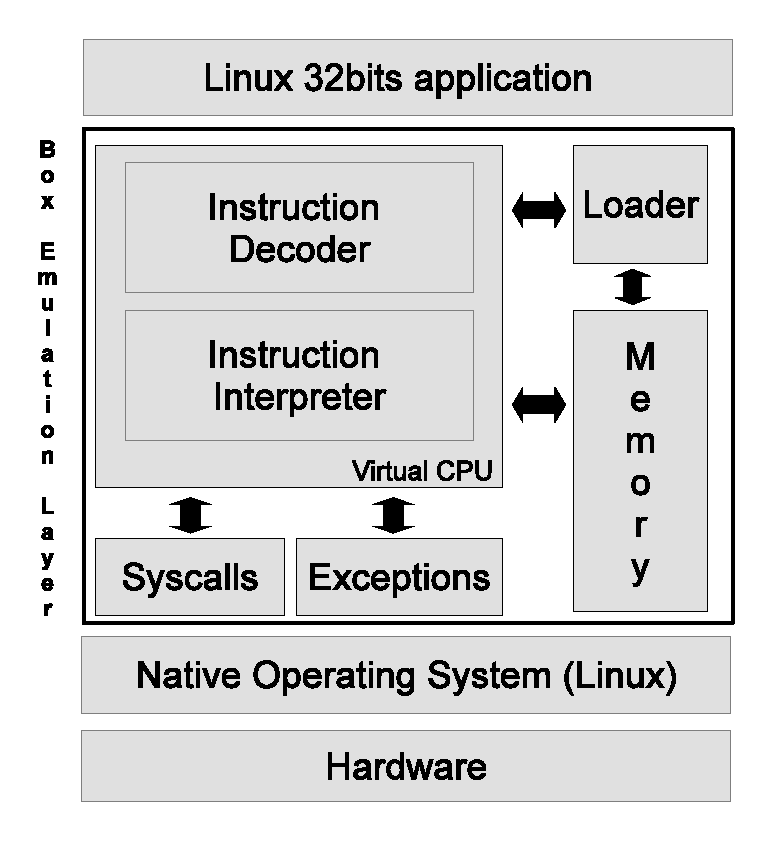
\includegraphics[width=0.5\columnwidth]{./figures/box-architecture.eps}
 \caption{Arquitetura do interpretador Box}
 \label{fig:box-architecture}
\end{figure}

A Figura \ref{fig:box-architecture} apresenta a arquitetura geral do interpretador, seguido da descrição de seus principais módulos.
Através deste interpretador, será possível carregar e interpretar um executável linux (elf) de 32bits com ligação dinâmica.

\begin{itemize}
 \item \textbf{Carregador} Responsável por ler e decodificar o executável principal e suas dependências, montar o espaço de endereçamento onde a interpretação ocorrerá e delegar o controle à CPU.
 \item \textbf{CPU} Módulo responsável por decodificar e interpretar (executar) as instruções x86 32 bits.
% \item \textbf{Decodificador} Neste passo implementaremos as rotinas de decodificação das instruções x86 32 bits.
% \item \textbf{Interpretador} Neste passo implementaremos as rotinas resposáveis por interpretar as instruções do x86 32 bits.
 \item \textbf{Memória} Módulo responsável pelo gerenciamento do espaço de memória reservado para a aplicação e suas dependências.
 \item \textbf{Syscalls} Rotinas que implementam as chamadas ao sistema operacional (\emph{system calls}) da ABI da aplicação sendo emulada (\emph{guest}).
 \item \textbf{Exceções} Módulo de gerenciamento de exceções da CPU (\emph{traps} e \emph{faults}).
\end{itemize}

\subsection{Otimização da máquina virtual}

Nesta etapa serão implementados os passos que adicionarão ao interpretador recursos de instrumentação e otimização de desempenho da interpretação.

\begin{itemize}
 \item \textbf{Otimização} Neste passo implementaremos uma das seguintes técnicas: DICache; Threaded-Interpretation; ou Pre-decoding.
 \item \textbf{Instrumentação} Neste passo implementaremos suporte para instrumentação dinâmica das aplicações emuladas.
\end{itemize}
 
\subsection{Análise de desempenho}

Nesta etapa serão conduzidas medições e análises de desempenho do sistema em relação ao emulador Bochs e será qunatificado o impacto das técnicas implementadas na etapa 2 no sistema.

\begin{itemize}
 \item \textbf{Desempenho 1} Neste passo avaliaremos o desempenho do sistema em relação ao emulador de sistema Bochs.
 \item \textbf{Desempenho 2} Neste passo iremos avaliar o efeito das técnicas implementadas na etapa 2 no desempenho do sistema.
\end{itemize}

\section{Cronograma}

%Será que precisamos de uma seção de resultados esperados e contribuições?

\section{Conclusão}

\begin{thebibliography}{99}

\bibitem{pin}Chi-Keung Luk, Robert Cohn, Robert Muth, Harish Patil, Artur
Klauser, Geoff Lowney, Steven Wallace, Vijay Janapa Reddi, Kim Hazelwood,
Pin: building customized program analysis tools with dynamic instrumentation, 
Proceedings of the 2005 ACM SIGPLAN conference on Programming language design
and implementation, June 12-15, 2005, Chicago, IL, USA 

\bibitem{hdtrans}Swaroop Sridhar, Jonathan S. Shapiro, Prashanth P. Bungale, 
HDTrans: a low-overhead dynamic translator, ACM SIGARCH Computer Architecture
News, v.35 n.1, p.135-140, March 2007 

\bibitem{dynamo}Bala, V., Duesterwald, E., and Banerjia, S. 1999. Transparent
dynamic optimization: The design and implementation of Dynamo. Hewlett Packard
Laboratories Technical Report HPL-1999-78. June 1999. 

\end{thebibliography}

\end{document}
